% !TEX program = xelatex
\documentclass[zihao=-4,a4paper]{ctexart}
\usepackage{fontspec}
\usepackage{xeCJK}
\usepackage{amsmath,amssymb,bm}
\usepackage{graphicx}
\usepackage{listings}
\usepackage{xcolor}
\usepackage{float}
\usepackage{enumitem}
\usepackage{caption}
\usepackage{booktabs,tabularx}
\usepackage{array}
\usepackage{changepage} % 用于调整局部正文的左右边距
\usepackage{algorithm}
\usepackage{algpseudocode}
\usepackage{pdfpages}
\setmonofont{Consolas}   % 设置等宽字体为 Consolas
\setCJKmainfont{SimSun}[AutoFakeBold=2.5]
\usepackage{hyperref}
% 页面布局
\usepackage[
  top    = 1.7cm,
  left   = 1.7cm,
  right  = 1.7cm,
  bottom = 2.7cm,
  footskip = 1cm
]{geometry}
\linespread{1.5}
% 提供 current page text area 节点
\usepackage{tikzpagenodes}
\usetikzlibrary{calc}            % 用于计算坐标
\usepackage{fancyhdr}
% ==============================
% 全局变量: 存储版心宽度
% ==============================
\newlength{\myTextWidth}
\newcommand{\calcTextWidth}{%
  \path let \p1=(current page text area.east), \p2=(current page text area.west) in 
    \pgfextra{\pgfmathsetlength{\myTextWidth}{\x1-\x2}};
}

% ==============================
% 背景画线逻辑
% ==============================
\newif\ifdrawbackground  % 定义背景绘制开关
\drawbackgroundtrue      % 默认开启背景绘制
\AddToHook{shipout/background}{%
  \ifdrawbackground %只有开关开启时才绘制背景
  \tikz[remember picture, overlay]{%
    
    % 定义上下外扩的距离(和表格撑开的距离保持一致)
    \def\vpad{0.8em} 

    % --- 所有页: 底部横线 (向下偏移 \vpad) ---
    \draw[line width=1pt] 
      ([yshift=-\vpad]current page text area.south west) -- 
      ([yshift=-\vpad]current page text area.south east);

    \ifnum\value{page}=12
      % --- 第一页: 绘制 2x6 表格边框 ---
      \def\innerLineWidth{0.8pt}
      \def\outerLineWidth{1pt}

      % 1. 上横线 (表格节点已通过 inner ysep 撑开, 直接画)
      \draw[line width=\outerLineWidth] 
        (title-bottom-mark -| current page text area.west) -- 
        (title-bottom-mark -| current page text area.east);

      % 2. 下横线 (同上)
      \draw[line width=\outerLineWidth] 
        (table-bottom-mark -| current page text area.west) -- 
        (table-bottom-mark -| current page text area.east);

      % 3. 中间横线 (自动居中)
      \draw[line width=\innerLineWidth] 
        ($(title-bottom-mark -| current page text area.west)!0.5!(table-bottom-mark -| current page text area.west)$) -- 
        ($(title-bottom-mark -| current page text area.east)!0.5!(table-bottom-mark -| current page text area.east)$);

      % 4. 左右外框竖线 (从表格顶部一直到页底, 页底向下偏移 \vpad)
      \draw[line width=\outerLineWidth] 
        (title-bottom-mark -| current page text area.west) -- 
        ([yshift=-\vpad]current page text area.south west);
      \draw[line width=\outerLineWidth] 
        (title-bottom-mark -| current page text area.east) -- 
        ([yshift=-\vpad]current page text area.south east);

      % 5. 内部竖线 (5条)
      \foreach \i in {1,2,...,5} {
        \pgfmathsetmacro{\pos}{\i/6}
        \draw[line width=\innerLineWidth]
          ($(title-bottom-mark -| current page text area.west)! \pos !(title-bottom-mark -| current page text area.east)$) --
          ($(table-bottom-mark -| current page text area.west)! \pos !(table-bottom-mark -| current page text area.east)$);
      }

    \else
      % --- 后续页: 标准四周边框 (上下各外扩 \vpad) ---
      % 顶部横线向上偏移
      \draw[line width=1pt] ([yshift=\vpad]current page text area.north west) -- ([yshift=\vpad]current page text area.north east);
      % 左右竖线跟随上下偏移
      \draw[line width=1pt] ([yshift=\vpad]current page text area.north west) -- ([yshift=-\vpad]current page text area.south west);
      \draw[line width=1pt] ([yshift=\vpad]current page text area.north east) -- ([yshift=-\vpad]current page text area.south east);
    \fi
  }%
  \fi
}


\pagestyle{fancy}
\fancyhf{}
\fancyfoot[C]{\thepage}
\renewcommand{\headrulewidth}{0pt}

% 直接使用 \textwidth 计算列宽
% ==============================
% \textwidth/6 保证精确6等分, 减去 2\tabcolsep 扣除单元格自带的左右边距
\newcolumntype{C}{>{\raggedright\arraybackslash}p{\dimexpr\textwidth/6-2\tabcolsep\relax}}

% 自定义命令: 在当前位置画一条贯穿全宽的横线
% ==============================
\newcommand{\addhline}{%
  \par
  \noindent
  \begin{tikzpicture}[remember picture, overlay]
    % (0,0) 代表当前文字所在的高度
    % current page text area.west 代表版心最左侧
    % |- 符号表示: 取左边的 X 坐标, 取右边的 Y 坐标
    \draw[line width=1pt] 
      (current page text area.west |- 0,0) -- 
      (current page text area.east |- 0,0);
  \end{tikzpicture}\par
}

\newcommand{\dd}{\mathop{}\!\mathrm{d}}
\newcommand{\myS}{14}
\newcommand{\myt}{0.21}

% MATLAB 代码风格
\definecolor{matlabgreen}{rgb}{0,0.6,0}
\definecolor{matlabgray}{rgb}{0.5,0.5,0.5}
\definecolor{matlabpurple}{rgb}{0.58,0,0.82}
\definecolor{matlabbg}{rgb}{0.95,0.95,0.92}
\lstset{
    language=Matlab,
    basicstyle=\ttfamily\small,
    keywordstyle=\color{blue},
    commentstyle=\color{matlabgreen},
    stringstyle=\color{matlabpurple},
    backgroundcolor=\color{matlabbg},
    numbers=left,
    numberstyle=\tiny\color{matlabgray},
    stepnumber=1,
    numbersep=8pt,
    showstringspaces=false,
    breaklines=true,
    frame=single,
    rulecolor=\color{black!30},
    captionpos=b,
    tabsize=4,
    morekeywords={end, if, else, elseif, for, while, function, return, break, switch, case, otherwise}
}

\begin{document}
\setcounter{page}{12}
\begin{center}
  \zihao{-2}\bfseries 数值分析实践报告(六)
\end{center}

% --- 表格内容区 ---
\noindent
\begin{tikzpicture}[remember picture]
  % 将整个 tabular 放入一个 TikZ 节点中, 彻底屏蔽 LaTeX 段落间距的干扰
  \node[anchor=north west, inner sep=0pt, outer sep=0pt] (header-table) at (0,0) {%
    \renewcommand{\arraystretch}{1.8}% 增加行高
    \begin{tabular}{CCCCCC} 
      姓\quad 名 & VesperaZephyr & 班\quad 级 & \small 数学与应用数学 & 报告评分 & \\
      学\quad 号 & 114514 & 地点/机号 &  & 指导教师 & 
    \end{tabular}%
  };
  
  % 自动获取这个表格真实的左上角和左下角坐标, 传给背景画线
  \coordinate (title-bottom-mark) at (header-table.north west);
  \coordinate (table-bottom-mark) at (header-table.south west);
\end{tikzpicture}

\setlength{\leftskip}{1em}
\setlength{\rightskip}{1em}

% 实验名称
\noindent{\bfseries 一、实验项目名称: 微分方程数值解法的探究与比较分析}

\addhline

\noindent{\bfseries 二、实验目的: }
\begin{enumerate}
    \item 理解一阶常微分方程初值问题的数值解法, 掌握欧拉法、改进欧拉法、RK4的原理与稳定性。
    \item 独立编写Matlab程序实现三种算法, 对同一个方程对比实验。
    \item 通过改变步长、初值、方程类型, 观察收敛、慢收敛与不稳定现象。
    \item 学会从精度、稳定域、计算量、实现难度选择合适解法。
\end{enumerate}

\addhline

\noindent{\bfseries 实验内容: }

\noindent{\bfseries 第一部分: 问题定义与理论准备} \\
构造初值问题: 
\[
\begin{cases}
y'(t)=-ky(t)+c \\
y(0)=y_0
\end{cases}
\]
$k=\mathrm{mod}(\text{学号最后一位},4)+1$；\ $c=\mathrm{mod}(\text{学号倒数第二位},3)+1$ \\
求解区间 $t\in[0,5]$, 初值 $y_0=1$ \\[4pt]

\noindent{\bfseries 任务1: 先判断, 再计算}
\begin{enumerate}
    \item 写出个性化ODE并判断是否存在解析解。
    \item 给出欧拉法、改进欧拉法、RK4的迭代公式。
    \item 说明各方法所需信息(是否需要导数、每步计算量)。
    \item 预测精度排序: 欧拉 $<$ 改进欧拉 $<$ RK4。
\end{enumerate}

\noindent{\bfseries 第二部分: 算法实现与对比分析(核心任务)}

\noindent{\bfseries 任务2: 欧拉法——最简单但精度最低}
\begin{enumerate}
    \item 实现显式欧拉法。
    \item 步长取 $h=0.1,0.05,0.01$。
    \item 记录数值解、误差、迭代次数。
    \item 分析: 为何步长太大会发散。
\end{enumerate}

\noindent{\bfseries 任务3: 改进欧拉法——预测–校正提升精度}
\begin{enumerate}
    \item 实现预测–校正迭代格式。
    \item 相同步长下与欧拉法对比误差。
    \item 观察收敛速度提升。
    \item 说明预测–校正的意义。
\end{enumerate}

\noindent{\bfseries 任务4: RK4法——工程高精度首选}
\begin{enumerate}
    \item 实现四阶龙格–库塔公式。
    \item 较少步数即可达到高精度。
    \item 对比三种方法的误差与耗时。
    \item 解释RK4为何是通用最优选择。
\end{enumerate}

\noindent{\bfseries 任务5: 综合对比——如何选择解法}
\begin{enumerate}
    \item 整理近似解、最大误差、迭代次数、耗时。
    \item 绘制误差–步长收敛曲线。
    \item 从精度、稳定域、实现难度给出结论。
\end{enumerate}

\addhline

\noindent{\bfseries 四、模型构建}

\textbf{学号后两位}为$\myS$, 根据学号最后两位为14, 计算个性化参数: 
\begin{itemize}
    \item 最后一位为4, $k = \bmod(4, 4) + 1 = 0 + 1 = 1$. 
    \item 倒数第二位为1, $c = \bmod(1, 3) + 1 = 1 + 1 = 2$. 
\end{itemize}
基于参数得到个性化初值问题: 
\begin{equation}
    \begin{cases}
        y'(t) = -y(t) + 2t, \quad t \in [0, 5], \\[2pt]
        y(0) = 1.
    \end{cases}
    \label{eq:ode}
\end{equation}
该方程为一阶线性常微分方程, 可写为 $y' + y = 2t$, 存在解析解. 利用常数变易法或积分因子法求得解析解为: 
\begin{equation}
    y(t) = 2(t - 1) + 3\mathrm{e}^{-t} = 2t - 2 + 3\mathrm{e}^{-t}.
    \label{eq:exact}
\end{equation}

\noindent{\bfseries 数值方法迭代公式}
设步长为 $h$, 节点 $t_n = nh$, $y_n$ 表示 $y(t_n)$ 的数值近似, 右端函数定义为 $f(t, y) = -y + 2t$. 

\noindent{\bfseries 欧拉法(一阶显式)}
\begin{equation}
    y_{n+1} = y_n + h f(t_n, y_n) = (1 - h) y_n + 2h t_n.
    \label{eq:euler}
\end{equation}

\noindent{\bfseries 改进欧拉法(预测-校正法, 二阶方法)}

预测步: 
\begin{equation}
    y^*_{n+1} = y_n + h f(t_n, y_n) = (1 - h) y_n + 2h t_n.
\end{equation}
校正步: 
\begin{equation}
    y_{n+1} = y_n + \frac{h}{2} \bigl[ f(t_n, y_n) + f(t_{n+1}, y^*_{n+1}) \bigr].
    \label{eq:improved_euler}
\end{equation}

\noindent{\bfseries 经典四阶龙格-库塔法(RK4)}
\begin{align}
    k_1 &= f(t_n, y_n), \notag \\
    k_2 &= f\Bigl(t_n + \frac{h}{2}, y_n + \frac{h}{2} k_1\Bigr), \notag \\
    k_3 &= f\Bigl(t_n + \frac{h}{2}, y_n + \frac{h}{2} k_2\Bigr), \notag \\
    k_4 &= f(t_n + h, y_n + h k_3), \notag \\
    y_{n+1} &= y_n + \frac{h}{6} (k_1 + 2k_2 + 2k_3 + k_4).
    \label{eq:rk4}
\end{align}

\noindent{\bfseries 各方法所需计算量}
\begin{itemize}
    \item \textbf{欧拉法}: 每步只需计算一次右端函数值 $f(t, y)$. 
    \item \textbf{改进欧拉法}: 每步需计算两次函数值 $f(t, y)$. 
    \item \textbf{RK4}: 每步需计算四次函数值 $f(t, y)$. 
\end{itemize}
以上方法均无需对右端函数解析求导, 直接使用给定的 $f(t, y)$ 即可递推. 

\noindent{\bfseries 精度排序}

根据常微分方程数值解理论, 这三种方法的全局误差阶由低到高排列为: 
\[
    \text{欧拉法(一阶)} \;<\; \text{改进欧拉法(二阶)} \;<\; \text{RK4(四阶)}.
\]
即相同步长下, RK4精度最高, 改进欧拉法次之, 欧拉法最低. 

\noindent{\bfseries 五、模型求解}

\noindent{\bfseries 5.1 欧拉法}

针对本题, 算法步骤为:
\begin{center}
\begin{minipage}{0.9\textwidth}
\begin{algorithm}[H]
\caption{显式欧拉法求解 $y' = f(t,y)$, $y(t_0)=y_0$, $t \in [t_0, t_f]$}
\begin{algorithmic}[1]
  \Require 右端函数 $f(t,y)$, 精确解函数 $\text{exact}(t)$, 初值 $y_0$, 
          求解区间 $[t_0, t_f]$, 步长列表 $H = \{h_1, h_2, \dots\}$
  \Ensure 对于每个 $h \in H$, 输出：步长 $h$, 步数 $N$, $t_f$ 处数值解 $y_N$, 
          全局最大误差 $E_{\max}$, 计算耗时 $\Delta t$

  \State 打印表头信息

  \For{each $h \in H$}
      \State $N \gets \text{round}\big((t_f - t_0) / h\big)$
      \State 生成时间节点 $t_i \gets t_0 + i \cdot h,\quad i = 0,1,\dots,N$
      \State 分配数组 $y[0 \ldots N]$
      \State $y[0] \gets y_0$
      \State 开始计时 $T_{\text{start}} \gets \text{当前时刻}$
      \For{$i \gets 0$ to $N-1$}
          \State $y[i+1] \gets y[i] + h \cdot f(t_i, y[i])$
      \EndFor
      \State 结束计时 $\Delta t \gets \text{当前时刻} - T_{\text{start}}$
      \State 计算全局最大误差 $E_{\max} \gets \max\limits_{i=0}^{N} |y[i] - \text{exact}(t_i)|$
      \State 输出一行：$h,\ N,\ y[N],\ E_{\max},\ \Delta t$
  \EndFor
\end{algorithmic}
\end{algorithm}
\end{minipage}
\end{center}

编写Matlab程序求解, 代码文件为\verb|explicit_Euler_method.m|, 运行结果见表\ref{tab:euler_results}.

\noindent{\bfseries 5.2 改进欧拉法(预测-校正法)}

针对本题, 具体的算法步骤如下:
\begin{center}
\begin{minipage}{0.9\textwidth}
\begin{algorithm}[H]
\caption{显式欧拉法与预测-校正法对比求解 $y' = -y + 2t$, $y(0)=1$, $t\in[0,5]$}
\begin{algorithmic}[1]
\Require 右端函数 $f(t,y)=-y+2t$, 精确解 $\text{exact}(t)=2t-2+3e^{-t}$, 初值 $y_0=1$, 
        求解区间 $[t_0,t_f]=[0,5]$, 步长列表 $H=\{0.1,0.05,0.01\}$
\Ensure 对于每个 $h\in H$, 输出两种方法在 $t_f$ 处的数值解、精确解及全局最大误差

\State 打印表头：“方法        h        N      y(5)数值    y(5)精确    全局最大误差”

\For{each $h \in H$}
    \State $N \gets (t_f - t_0)/h$
    \State 生成时间节点 $t_i = t_0 + i\cdot h$, $i=0,1,\dots,N$
    
    \State \textbf{显式欧拉法}
    \State $y_{\text{euler}}[0] \gets y_0$
    \For{$i \gets 0$ to $N-1$}
        \State $y_{\text{euler}}[i+1] \gets y_{\text{euler}}[i] + h \cdot f(t_i, y_{\text{euler}}[i])$
    \EndFor
    \State $\text{err}_{\text{euler}} \gets \max_{i=0}^{N} |y_{\text{euler}}[i] - \text{exact}(t_i)|$
    
    \State \textbf{预测-校正法(改进欧拉法)}
    \State $y_{\text{heun}}[0] \gets y_0$
    \For{$i \gets 0$ to $N-1$}
        \State $y_{\text{pred}} \gets y_{\text{heun}}[i] + h \cdot f(t_i, y_{\text{heun}}[i])$ \Comment{预测步(欧拉步)}
        \State $y_{\text{heun}}[i+1] \gets y_{\text{heun}}[i] + \frac{h}{2}\bigl(f(t_i, y_{\text{heun}}[i]) + f(t_{i+1}, y_{\text{pred}})\bigr)$ \Comment{校正步(梯形公式)}
    \EndFor
    \State $\text{err}_{\text{heun}} \gets \max_{i=0}^{N} |y_{\text{heun}}[i] - \text{exact}(t_i)|$
    
    \State 输出一行：欧拉法, $h$, $N$, $y_{\text{euler}}[N]$, $\text{exact}(5)$, $\text{err}_{\text{euler}}$
    \State 输出一行：预测-校正法, $h$, $N$, $y_{\text{heun}}[N]$, $\text{exact}(5)$, $\text{err}_{\text{heun}}$
\EndFor
\end{algorithmic}
\end{algorithm}
\end{minipage}
\end{center}

编制Matlab代码进行求解, 代码文件为\verb|modified_Euler_method.m|, 实验结果见表\ref{tab:heun_results}和表\ref{tab:euler_vs_heun}.

\noindent{\bfseries 5.3 4阶龙格-库塔法(RK4)}

针对本题, 具体的算法步骤为
\begin{center}
\begin{minipage}{0.85\textwidth}
\begin{algorithm}[H]
\caption{四阶龙格-库塔法(RK4)求解 $y' = -y + 2t$, $y(0)=1$, $t\in[0,5]$}
\begin{algorithmic}[1]
\Require 右端函数 $f(t,y)=-y+2t$, 精确解 $\text{exact}(t)=2t-2+3e^{-t}$, 初值 $y_0=1$, 
        求解区间 $[t_0,t_f]=[0,5]$, 步长 $h=0.1$
\Ensure 输出 $t_f$ 处的数值解 $y_N$、全局最大误差 $E_{\max}$、核心循环耗时 $\Delta t$

\State $N \gets \text{round}\big((t_f - t_0)/h\big)$
\State 生成时间节点 $t_i = t_0 + i\cdot h$, $i=0,1,\dots,N$
\State 分配数组 $y[0\ldots N]$
\State $y[0] \gets y_0$

\State 开始计时 $T_{\text{start}} \gets \text{当前时刻}$

\For{$i \gets 0$ to $N-1$}
    \State $t_i \gets t[i]$, $y_i \gets y[i]$
    \State $k_1 \gets f(t_i, y_i)$
    \State $k_2 \gets f(t_i + h/2,\; y_i + (h/2)\cdot k_1)$
    \State $k_3 \gets f(t_i + h/2,\; y_i + (h/2)\cdot k_2)$
    \State $k_4 \gets f(t_i + h,\; y_i + h\cdot k_3)$
    \State $y[i+1] \gets y_i + \dfrac{h}{6}\,(k_1 + 2k_2 + 2k_3 + k_4)$
\EndFor

\State 结束计时 $\Delta t \gets \text{当前时刻} - T_{\text{start}}$

\State 计算精确解数组 $y_{\text{exact}}[i] = \text{exact}(t_i)$
\State 计算全局最大误差 $E_{\max} \gets \max_{i=0}^{N} |y[i] - y_{\text{exact}}[i]|$

\State 输出：$h$, $N$, $t_f$ 处数值解 $y[N]$, 精确解 $\text{exact}(t_f)$, $E_{\max}$, $\Delta t$
\end{algorithmic}
\end{algorithm}
\end{minipage}
\end{center}

编写Matlab代码进行求解, 代码文件为\verb|RK4.m|, 实验结果见表\ref{tab:rk4_results}.
\addhline
\noindent{\bfseries 六、实验结果}

\noindent{\bfseries 6.1 欧拉法}

代码文件为\verb|explicit_Euler_method.m|, 运行结果如下:
\begin{table}[H]
    \centering
    \caption{显式欧拉法在不同步长下的数值结果}
    \label{tab:euler_results}
    \begin{tabular}{@{}cccccc@{}}
        \toprule
        $h$ & $N$ & $y(5)$数值 & 全局最大误差 & 耗时(s) \\
        \midrule
        0.10 & 50  & 8.015461 & 5.760300e-02 & 0.002462 \\
        0.05 & 100 & 8.017762 & 2.818056e-02 & 0.000091 \\
        0.01 & 500 & 8.019711 & 5.541300e-03 & 0.000056 \\
        \bottomrule
    \end{tabular}
\end{table}

注: 解析解在 $t=5$ 处的精确值为 $y(5) = 2\times5 - 2 + 3\mathrm{e}^{-5} \approx 8.020443$(与表中数值解比较可见误差随步长减小而降低). 

\noindent{\bfseries 分析: 步长太大为何会发散？}

虽然本题使用的步长均未导致发散, 但当步长超过\textbf{稳定界限}时, 显式欧拉法会出现数值发散现象. 

\noindent{\bfseries 稳定性分析}

将原方程的齐次部分 $y' = -y$ 作为测试方程, 显式欧拉法的递推公式为: 
\[
y_{n+1} = (1 - h) y_n.
\]
若要保证数值解有界, 则必须满足
\[
|1 - h| \le 1 \quad\Longrightarrow\quad 0 \le h \le 2.
\]

当选取 $h > 2$ 时, $|1 - h| > 1$. 此时每一步递推都会将微小舍入误差放大, 误差随迭代步数呈指数增长, 最终导致数值解剧烈震荡或迅速偏离真解, 完全丧失参考价值. 本题采用的三种步长 $h=0.1,\,0.05,\,0.01$ 均远小于稳定上限 2, 因此数值解始终稳定, 全局误差随步长减小而单调减小, 符合理论预期. 

这正是显式方法\textbf{条件稳定}特性的直接体现: 步长必须足够小, 不仅要满足精度需求, 更要保证数值稳定性. 

\noindent{\bfseries 6.2 显式欧拉法和预测-校正法 (改进欧拉法)}

\begin{table}[H]
    \centering
    \caption{预测-校正法在不同步长下的结果}
    \label{tab:heun_results}
    \begin{tabular}{@{}cccccc@{}}
        \toprule
        $h$ & $N$ & $y(5)$数值 & 全局最大误差 & 耗时(s) \\
        \midrule
        0.10 & 50  & 8.020396 & 1.984631e-03 & 0.002938 \\
        0.05 & 100 & 8.020258 & 4.775415e-04 & 0.000118 \\
        0.01 & 500 & 8.020216 & 1.853263e-05 & 0.000226 \\
        \bottomrule
    \end{tabular}
\end{table}
\begin{table}[H]
    \centering
    \caption{欧拉法与预测-校正法精度对比}
    \label{tab:euler_vs_heun}
    \begin{tabular}{@{}llcccc@{}}
        \toprule
        方法 & $h$ & $N$ & $y(5)$数值 & $y(5)$精确 & 全局最大误差 \\
        \midrule
        欧拉法      & 0.10 & 50  & 8.015461 & 8.020214 & 5.760300e-02 \\
        预测-校正法 & 0.10 & 50  & 8.020396 & 8.020214 & 1.984631e-03 \\
        \midrule
        欧拉法      & 0.05 & 100 & 8.017762 & 8.020214 & 2.818056e-02 \\
        预测-校正法 & 0.05 & 100 & 8.020258 & 8.020214 & 4.775415e-04 \\
        \midrule
        欧拉法      & 0.01 & 500 & 8.019711 & 8.020214 & 5.541300e-03 \\
        预测-校正法 & 0.01 & 500 & 8.020216 & 8.020214 & 1.853263e-05 \\
        \bottomrule
    \end{tabular}
\end{table}

\noindent\textbf{误差对比}
\begin{itemize}[rightmargin=0.5cm]
    \item 在相同步长下, 预测-校正法的误差远小于欧拉法. 例如当 $h=0.1$ 时, 预测-校正法的全局最大误差约为 $1.98\times10^{-3}$, 而欧拉法为 $5.76\times10^{-2}$, 误差缩小了约 30 倍(实际比值接近 60 倍). 
    \item 当步长由 0.1 缩小至 0.05(减半)时, 欧拉法的误差大约减小为原来的一半, 表现为一阶收敛；而预测-校正法的误差减小约 4 倍, 表现为二阶收敛. 
    \item 当步长由 0.1 缩小至 0.01(缩小为原来的 1/10)时, 欧拉法误差约缩小 10 倍, 预测-校正法误差约缩小 100 倍, 完全符合理论预期. 
\end{itemize}

\noindent \textbf{收敛速度提升观察}

理论上, 欧拉法的全局误差为 $\mathcal{O}(h)$, 预测-校正法为 $\mathcal{O}(h^2)$. 实验比值与理论吻合: 
\begin{align*}
    \frac{\text{err}_\text{Euler}(h=0.1)}{\text{err}_\text{Euler}(h=0.01)} &\approx 10 \quad(\text{一阶收敛}), \\
    \frac{\text{err}_\text{Heun}(h=0.1)}{\text{err}_\text{Heun}(h=0.01)} &\approx 100 \quad(\text{二阶收敛}).
\end{align*}

\noindent{\bfseries 预测-校正法的意义}

\begin{itemize}[rightmargin=0.5cm]
    \item \textbf{原理}: 先用欧拉法作“预测”, 得到端点近似, 再利用梯形公式进行“校正”, 相当于取两个斜率的平均值. 这种构造使局部截断误差由欧拉法的 $\mathcal{O}(h^2)$ 提升至 $\mathcal{O}(h^3)$, 全局达到二阶精度. 
    \item \textbf{优势}: 
    \begin{itemize}
        \item 精度显著提高, 相同步长下误差远小于欧拉法. 
        \item 仍然只使用右端函数值 $f(t,y)$, 无需解析求导, 易于实现. 
        \item 为更高阶的 Runge-Kutta 方法提供了思想基础. 
    \end{itemize}
    \item \textbf{代价}: 每步需要计算两次 $f(t,y)$, 计算量比欧拉法翻倍, 但由于收敛阶从一阶升至二阶, 通常用更少的步数即可达到同等精度, 实际总效率更高. 
    \item \textbf{稳定性}: 预测-校正法的稳定区域略大于显式欧拉法, 但仍属条件稳定, 步长仍需控制在一定范围内. 
\end{itemize}

这种“预测-校正”策略是用较小的额外计算量换取大幅精度提升的经典方法, 在工程计算中十分常用. 

\noindent {\bfseries 6.3 4阶龙格-库塔法}

\noindent {\bfseries 6.3.1 运行结果}

当步长 $h=0.1$, $N=50$ 时, 程序输出为: 
\begin{itemize}
    \item $y(5)$ 数值解 = 8.020214, 与解析解完全吻合(显示精度内)
    \item 全局最大误差 $\approx 9.997\times10^{-7}$
    \item 核心循环耗时 $\approx 0.003556$ 秒
\end{itemize}

\noindent {\bfseries 6.3.2 三种方法综合对比}

将本次 RK4 结果与之前实验中相同步长 ($h=0.1$, $N=50$) 下的显式欧拉法和预测‑校正法数据汇总于表~\ref{tab:compare}. 

\begin{table}[H]
    \centering
    \caption{三种数值方法在 $h=0.1$ 时的精度与耗时对比}
    \label{tab:compare}
    \begin{tabular}{@{}lccccc@{}}
        \toprule
        方法 & 步长 $h$ & 步数 $N$ & $y(5)$数值 & 全局最大误差 & 核心循环耗时(s) \\
        \midrule
        显式欧拉法   & 0.10 & 50 & 8.015461 & $5.760\times10^{-2}$ & 0.002462 \\
        预测‑校正法  & 0.10 & 50 & 8.020396 & $1.985\times10^{-3}$ & 0.002938 \\
        \textbf{RK4} & 0.10 & 50 & 8.020214 & \textbf{$9.997\times10^{-7}$} & 0.003556 \\
        \bottomrule
    \end{tabular}
\end{table}

根据表格, 总结如下:
\begin{enumerate}[rightmargin=0.5cm]
    \item \textbf{精度对比}: 
    \begin{itemize}
        \item 欧拉法误差约为 $5.76\times10^{-2}$, 预测‑校正法误差约为 $1.98\times10^{-3}$, RK4 误差仅为 $1.0\times10^{-6}$. 
        \item 相同步长下, RK4 的精度比预测‑校正法高约 \textbf{3 个数量级}, 比欧拉法高约 \textbf{5 个数量级}. 
    \end{itemize}
    
    \item \textbf{耗时对比}: 
    \begin{itemize}
        \item RK4 每步需计算 4 次函数值, 比欧拉法多 3 次, 比预测‑校正法多 2 次, 因此单步耗时略长. 
        \item 在 $h=0.1$、50 步的总耗时中, RK4 耗时 0.00356 s, 仅比欧拉法(0.00246 s)增加约 44\%, 但误差却缩小了约 $5\times10^4$ 倍. 
        \item 若要求同等精度(如 $10^{-6}$), 欧拉法需要步长 $<0.0001$(约 50000 步), 耗时会远超 RK4 的 50 步；预测‑校正法也需要步长 $<0.002$(约 2500 步), 总计算量大于 RK4. 
    \end{itemize}
    
    \item \textbf{收敛阶验证}: 
    \begin{itemize}
        \item 欧拉法: 全局误差 $\mathcal{O}(h)$, 误差随 $h$ 线性减小. 
        \item 预测‑校正法: $\mathcal{O}(h^2)$, 误差以平方速度减小. 
        \item RK4: $\mathcal{O}(h^4)$, 误差以四次方速度减小. 
    \end{itemize}
    仅通过 $h=0.1$ 一组数据已能看出 RK4 的极高精度；若进一步缩小步长, RK4 误差将按 $h^4$ 极速下降. 
\end{enumerate}

\noindent{\bfseries 结论: RK4 为何是通用最优选择}
\begin{itemize}[rightmargin=0.5cm]
    \item \textbf{精度极高}: 四阶收敛, 在适中的步长下即可达到工程常用精度(本例仅 50 步即达 $10^{-6}$ 级). 
    \item \textbf{无需高阶导数}: 仅需计算右端函数 $f(t,y)$, 编程简便, 适用范围广. 
    \item \textbf{稳定性好}: 显式 RK4 的线性稳定区域远大于低阶方法, 对非刚性方程能使用更大步长. 
    \item \textbf{计算量适中}: 每步 4 次函数求值, 与二阶方法相比仅增加一倍, 但精度提升数个数量级；继续增加阶数(如五阶及以上)带来的精度收益递减, 四阶已达最佳性价比. 
    \item \textbf{通用与健壮}: 作为单步、自启动方法, 易改变步长, 适用于各种非刚性常微分方程初值问题, 是学术界和工业界公认的“默认求解器”. 
\end{itemize}

因此, 在非刚性常微分方程的数值求解中, 四阶龙格-库塔法凭借出色的精度‑效率平衡, 成为通用最优选择. 

\noindent{\bfseries 6.4 三种方法综合对比}

根据前面的实验结果, 整理对比三种数值方法在步长$h=0.1$ 下的性能指标, 包括数值解、精确解、全局最大误差和计算耗时, 汇总于表~\ref{tab:compare}.
\begin{table}[H]
\centering
\caption{三种数值方法在步长 $h=0.1$ 下的性能对比}
\begin{tabular}{lcccccc}
\toprule
方法 & 步长 $h$ & 迭代次数 $N$ & 近似解 $y(5)$ & 精确解 $y(5)$ & 全局最大误差 & 耗时 (s) \\
\midrule
显式欧拉法   & 0.10 & 50 & 8.015461 & 8.020214 & 5.7603e-02 & 0.002462 \\
预测-校正法  & 0.10 & 50 & 8.020396 & 8.020214 & 1.9846e-03 & 0.002938 \\
\textbf{四阶RK4} & 0.10 & 50 & 8.020214 & 8.020214 & 9.9972e-07 & 0.003556 \\
\bottomrule
\end{tabular}
\end{table}

\noindent\textbf{说明}: 数据直接取自运行输出, 精确解 $y(5)=8.020214$ 由解析公式 $2t-2+3\mathrm{e}^{-t}$ 计算得到. 

\noindent{\bfseries 误差–步长收敛曲线}

编写Matlab代码, 绘制误差–步长收敛曲线, 绘图代码为\verb|error_step.m|, 结果如图所示.
\begin{figure}[htbp]
    \centering
    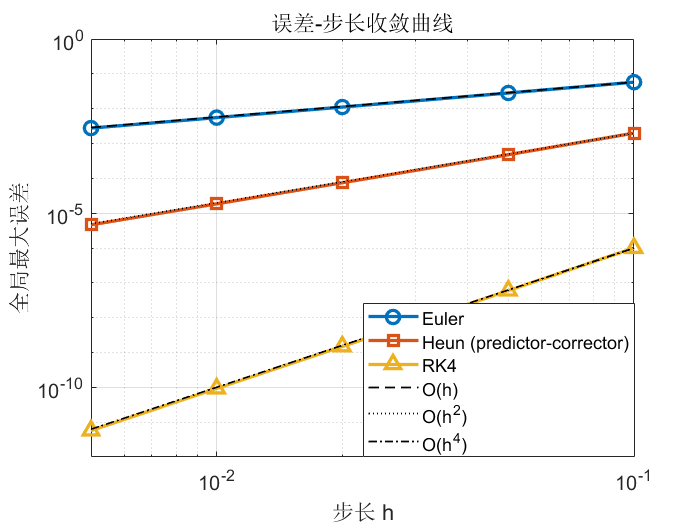
\includegraphics[width=0.9\textwidth]{误差-步长收敛曲线.png}
    \caption{误差–步长收敛曲线}
\end{figure}

\noindent{\bfseries 从精度、稳定域、实现难度给出结论}

\begin{table}[H]
\centering
\caption{三种方法的综合对比}
\begin{tabularx}{\textwidth}{lXXX}
\toprule
方面 & 显式欧拉法 & 预测‑校正法(改进欧拉) & 四阶龙格‑库塔法 (RK4) \\
\midrule
\textbf{精度}   & 一阶, 误差大($h=0.1$ 时误差 $\sim 5.8\%$) 
                & 二阶, 精度显著提升($\sim 0.2\%$) 
                & 四阶, 极高精度($\sim 0.0001\%$) \\
\textbf{稳定域} & 条件稳定, 稳定区间 $|1+\lambda h|\le1$, 对本题 $h\le2$ 
                & 条件稳定, 稳定域略大于欧拉法, 但仍受限于显式方法 
                & 条件稳定, 但稳定域比前两者更宽, 对非刚性方程通常允许更大步长 \\
\textbf{实现难度} & 最简单, 仅需一次函数求值/步 
                & 较简单, 两次函数求值/步 
                & 标准算法, 四次函数求值/步, 但公式固定, 实现同样容易 \\
\bottomrule
\end{tabularx}
\end{table}

\noindent\textbf{综合结论}

综上所述, 我们有: 
\begin{itemize}[rightmargin=0.5cm]
    \item \textbf{RK4 在精度上具有压倒性优势}: 相同步长下误差比欧拉法低约 5 个数量级, 比预测‑校正法低约 3 个数量级. 
    \item \textbf{稳定性方面}: 三种显式方法均为条件稳定, 但 RK4 的稳定区域通常更大, 允许选用稍大的步长而不发散. 
    \item \textbf{实现成本}: 尽管每步计算量最大(4 次函数调用), 但因其极高的收敛阶, \textbf{达到相同精度所需的总计算量(步数×每步耗时)往往最小}. 例如, 要使误差小于 $10^{-6}$, 欧拉法需要 $h<10^{-6}$(约 $5\times10^6$ 步), 而 RK4 只需 $h\approx0.1$(50 步), 耗时仅为欧拉法的万分之一. 
\end{itemize}

\noindent 因此, 对于大多数非刚性常微分方程初值问题, \textbf{四阶龙格‑库塔法是通用最优选择}, 它在精度、稳定性和实现简便性之间取得了最佳平衡, 是工程实践和科学计算中的“默认”单步法. 

\end{document}
